\chapter{Исследовательская часть}
В этом разделе будет приведена демострация работы программы, 
а также исследовано время работы алгоритмов.

\section{Демонстрация работы программы}
На рисунке 4.1 показана демонстрация работы программы.

\begin{figure}[hp]
	\begin{center}
		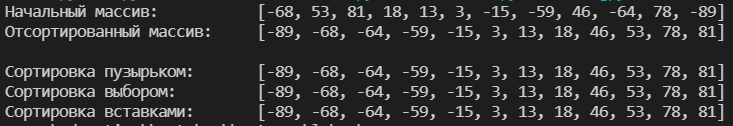
\includegraphics[width=\linewidth]{inc/work.png}
	\end{center}
	\caption{Демонстрация работы программы}
\end{figure}

\section{Технические характеристики}
Технические характеристики устройства, на котором выполнялось тестирование, следующие:
\begin{itemize}
	\item операционная система: Windows 10;
	\item память: 8 GB;
	\item процессор: Intel Core i5-1135G7 @ 2.40GHz \cite{intel}.
\end{itemize}

Во время тестирования ноутбук был нагружен только встроенными приложениями окружения, а также непосредственно системой тестирования.


\section{Время работы программы}
Для замера времени работы алгоритмов рассматривалось три случая:
\begin{enumerate}
	\item Массив, состоящий из случайных чисел.
	\item Отсортированный массив.
	\item Массив, сортированный в обратном порядке.
\end{enumerate}

\subsection{Сравнение времени работы алгоритмов на массиве случайных чисел}
В таблице 4.1 приведены результаты тестирования работы алгоритмов на массиве случайных чисел.
В первом столбце указан размер массива, а в следующих трёх -- время работы для каждой
реализации алгоритмов сортировки.

\FloatBarrier
\begin{table}[h]
	\caption{Результаты тестов на массиве случайных чисел}
	\centering
	\begin{tabular}{ | l | l | l | l |}
		\hline
		Размер массива & BubbleSort & SelectSort & InsertSort \\ \hline
		1 & 7812 & 9375 & 4687 \\
		5 & 20312 & 21875 & 12500 \\
		10 & 50000 & 67187 &  37500 \\
		20 & 201562 & 154687 & 106250 \\
		50 & 1284375 & 832812 & 795312 \\
		75 & 2660937 & 1798437 & 1478125 \\
		100 & 4468750 & 3156250 & 2515625 \\
		250 & 29375000 & 17578125 & 17109375 \\
		500 & 117187500 & 68906250 & 60937500 \\
		1000 & 476406250 & 276718750 & 257343750 \\
		\hline
	\end{tabular}
\end{table}
\FloatBarrier

На рисунке 4.2 изображены графики времени работы алгоритмов на массиве случайных чисел.
График был построен в логарифмической шкале, так как сортировка вставками в сотни раз быстрее, чем
остальные реализации, поэтому в обычной шкале график напоминает горизонтальную линию около нуля.

\FloatBarrier
\begin{figure}[h]
	\begin{center}
		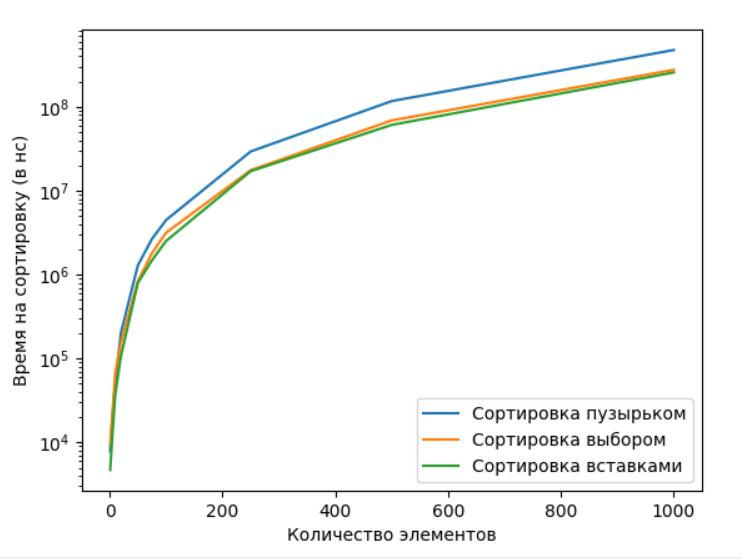
\includegraphics[]{inc/random1.png}
	\end{center}
	\caption{График зависимости времени сортировки от количества элементов в массиве для массива случайных чисел}
\end{figure}
\FloatBarrier

Также на рисунке 4.3 приведено сравнение сортировки пузырьком и сортировки выбором, так как 
по порядку они схожи.

\FloatBarrier
\begin{figure}[h]
	\begin{center}
		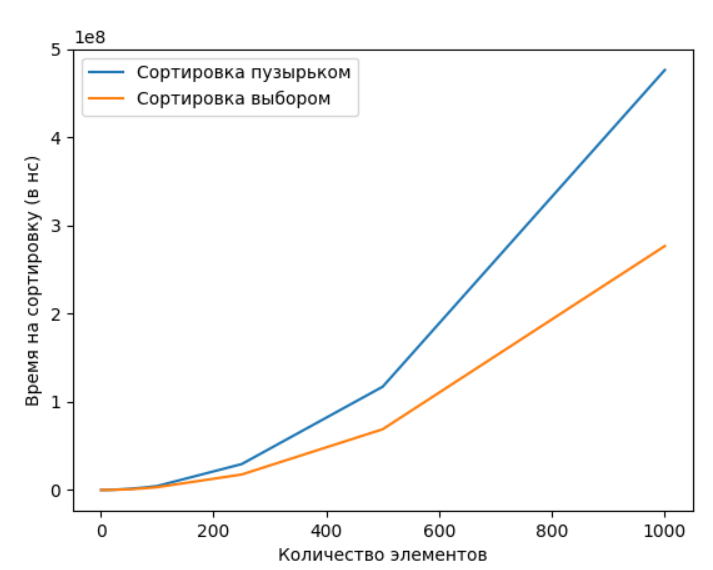
\includegraphics[]{inc/random2.png}
	\end{center}
	\caption{График зависимости времени сортировки от количества элементов в массиве для массива случайных чисел}
\end{figure}
\FloatBarrier

\subsection{Сравнение времени работы алгоритмов на отсортированном массиве}
В таблице 4.2 приведены результаты тестирования работы алгоритмов на отсортированном массиве.
В первом столбце указан размер массива, а в следующих трёх -- время работы для каждой
реализации алгоритмов сортировки.

\FloatBarrier
\begin{table}[h]
	\caption{Результаты тестов на отсортированном массиве}
	\centering
	\begin{tabular}{ | l | l | l | l |}
		\hline
		Размер массива & BubbleSort & SelectSort & InsertSort \\ \hline
		1 & 7812 & 9375 & 4687 \\
		5 & 17187 & 23437 & 12500 \\
		10 & 42187 & 54687 &  15625 \\
		20 & 137500 & 160937 & 31250 \\
		50 & 795312 & 801562 & 71875 \\
		75 & 1682812 & 1715625 & 107812 \\
		100 & 2984375 & 2937500 & 140625 \\
		250 & 18828125 & 18359375 & 390625 \\
		500 & 72968750 & 70937500 & 625000 \\
		1000 & 295625000 & 275937500 & 1562500 \\
		\hline
	\end{tabular}
\end{table}
\FloatBarrier

На рисунке 4.4 изображены графики времени работы алгоритмов на отсортированном массиве.
График был построен в логарифмической шкале, так как сортировка вставками в сотни раз быстрее, чем
остальные реализации, поэтому в обычной шкале график напоминает горизонтальную линию около нуля.

\FloatBarrier
\begin{figure}[h]
	\begin{center}
		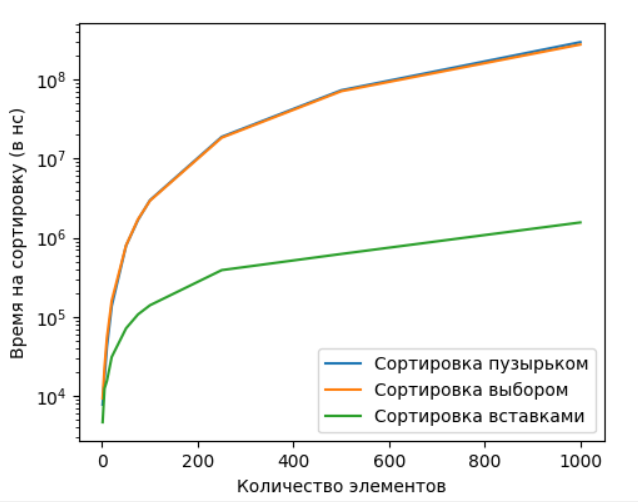
\includegraphics{inc/random3.png}
	\end{center}
	\caption{График зависимости времени сортировки от количества элементов в массиве для отсортированного массива}
\end{figure}
\FloatBarrier

Также на рисунке 4.5 приведено сравнение сортировки пузырьком и сортировки выбором, так как 
по порядку они схожи.

\FloatBarrier
\begin{figure}[h]
	\begin{center}
		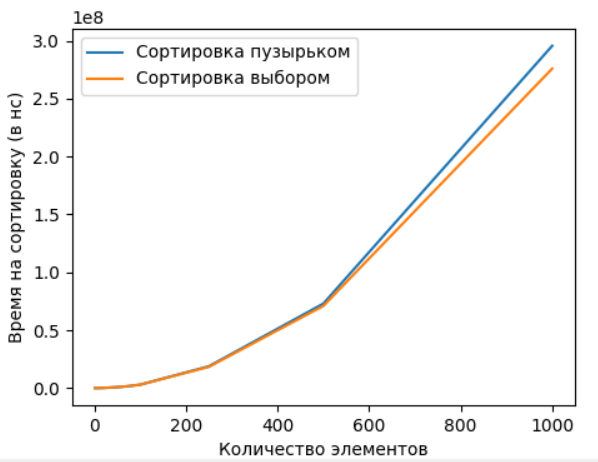
\includegraphics{inc/random4.png}
	\end{center}
	\caption{График зависимости времени сортировки от количества элементов в массиве для массива случайных чисел}
\end{figure}
\FloatBarrier

\subsection{Сравнение времени работы алгоритмов на обратно сортированном массиве}

В таблице 4.3 приведены результаты тестирования работы алгоритмов на массиве, сортированном в обратном порядке.
В первом столбце указан размер массива, а в следующих трёх -- время работы для каждой
реализации алгоритмов сортировки.

\FloatBarrier
\begin{table}[h]
	\caption{Результаты тестов массиве, отсортированном в обратном порядке}
	\centering
	\begin{tabular}{ | l | l | l | l |}
		\hline
		Размер массива & BubbleSort & SelectSort & InsertSort \\ \hline
		1 & 6250 & 9375 & 4687 \\
		5 & 25000 & 26562 & 21875  \\
		10 & 75000 & 67187 & 68750 \\
		20 & 282812 & 179687 & 218750 \\
		50 & 1629687 & 954687 & 1240625 \\
		75 & 3625000 & 2104687 & 3003125 \\
		100 & 6687500 & 3734375 & 5015625 \\
		250 & 39453125 & 21796875 & 29921875 \\
		500 & 170468750 & 89218750 & 122812500 \\
		1000 & 671875000 & 342031250 & 523750000 \\
		\hline
	\end{tabular}
\end{table}
\FloatBarrier

На рисунке 4.6 изображены графики времени работы алгоритмов на массиве, отсортированном в обратном порядке.
График был построен в логарифмической шкале, так как сортировка вставками в сотни раз быстрее, чем
остальные реализации, поэтому в обычной шкале график напоминает горизонтальную линию около нуля.

\FloatBarrier
\begin{figure}[ht]
	\begin{center}
		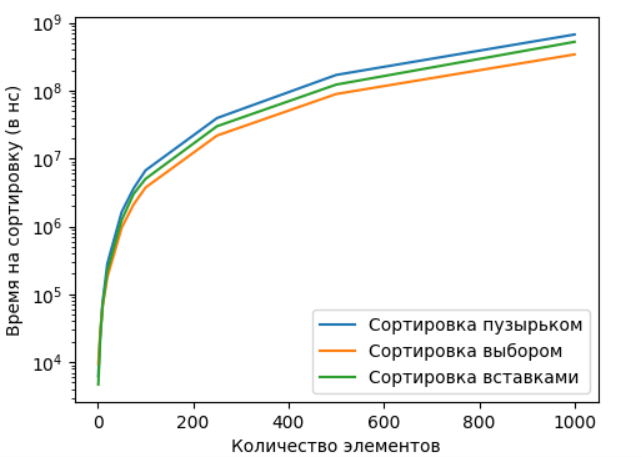
\includegraphics{inc/random5.png}
	\end{center}
	\caption{График зависимости времени сортировки от количества элементов в массиве для массива случайных чисел}
\end{figure}
\FloatBarrier

Также на рисунке 4.7 приведено сравнение сортировки пузырьком и сортировки выбором, так как 
по порядку они схожи.

\FloatBarrier
\begin{figure}[ht]
	\begin{center}
		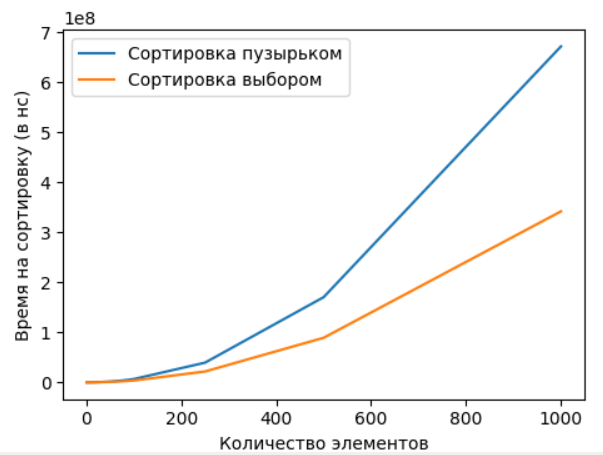
\includegraphics{inc/random6.png}
	\end{center}
	\caption{График зависимости времени сортировки от количества элементов в массиве для массива случайных чисел}
\end{figure}
\FloatBarrier

\section{Вывод} 
Для массива, состоящих из случайных чисел, сортировка вставками показала лучшие результаты на всех N.
Сортировка пузырьком показала самый медленный результат, выполняясь при $N = 1000$ почти в два раза дольше,
чем остальные способы.

Для уже отсортированного массива сортировка вставками оказалась при $N = 1000$ в 250 раз быстрее, чем
другие сортировки. Тем самым подтвердилось, что в лучшем случае сортировка вставками
работает быстрее, чем остальные, так как её порядок - $O(N)$, а для других сортировок - $O(N^2)$.
Результаты сортировки выбором почти не отличаются от результатов при массиве, состоящих из случайных чисел.
Сортировка пузырьком происходила в полтора раза быстрее, чем при массиве случайных чисел, но и в этом
случае она была самой медленной.

Для массива, сортированном в обратном порядке, сортировка выбором оказалась самым быстрым вариантом,
превзойдя при $N = 1000$ в полтора раза сортировку вставками и в два раза - сортировку пузырьком.

Тем самым подтвердились следующие оценки трудоёмкости:
\begin{itemize}
	\item сортировка вставками в лучшем случае работает на порядок быстрее, чем остальные способы;
	\item сортировка выбором оказалась быстрее всех при худшем случае, при оценке трудоёмкоси ей коэффициент перед $N^2$ был наименьшим.
\end{itemize} 